\begin{center}
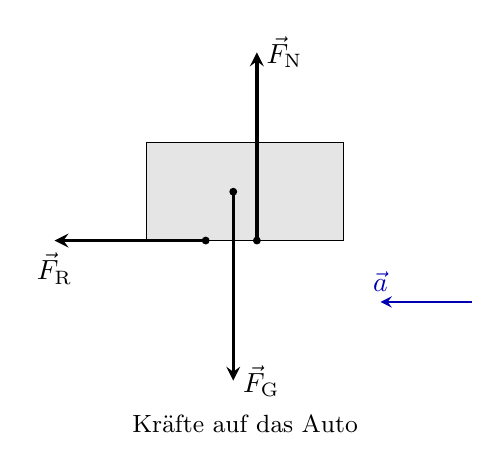
\begin{tikzpicture}[>=stealth]
 \draw[fill=gray!20] (-1.25,-0.62) rectangle (1.25,0.62);
 \draw[->, very thick] (-0.15,0) -- (-0.15,-2.4);
 \fill (-0.15,0) circle (0.05);
 \node[right] at (-0.15,-2.4) {$\vec F_\mathrm{G}$};
 \draw[->, very thick] (0.15,-0.62) -- (0.15,1.77);
 \fill (0.15,-0.62) circle (0.05);
 \node[right] at (0.15,1.77) {$\vec F_\mathrm{N}$};
 \draw[->, very thick] (-0.5,-0.62) -- (-2.42,-0.62);
 \fill (-0.5,-0.62) circle (0.05);
 \node[below=1pt] at (-2.42,-0.62) {$\vec F_\mathrm{R}$};
 \draw[->, thick, blue!70!black] (2.88,-1.4) -- (1.72,-1.4) node[above] {$\vec a$};
 \node[font=\small] at (0,-2.95) {Kräfte auf das Auto};
\end{tikzpicture}
\end{center}

\begin{abcliste}
\abc
Die einzige waagrechte Kraft auf das Auto ist die Reibung der Strasse an den Reifen: höchstens $\mu_\mathrm{H}$ mal die Normalkraft. Auf ebener Strasse ist die Normalkraft gleich der Gewichtskraft:
\begin{align}
 \ssc{F}{R} &= \FRF \\
   &= \muH\cdot\m\cdot\g \\
   &= \FR \approx \result{\FRP{3}{2}}
\end{align}
Die Verzögerung folgt aus dem Aktionsprinzip:
\begin{align}
 a &= \frac{\ssc{F}{R}}{m} = \aF \\
   &= \muH\cdot\g \\
   &= \a \approx \result{\aP{0}{2}}
\end{align}

\abc
Nein. Die Masse kürzt sich weg: Ein schwereres Auto braucht mehr Bremskraft, aber die Strasse liefert entsprechend mehr. Es hält nicht früher an (in Wirklichkeit entscheiden Reifen und Bremsen).
\end{abcliste}
